\documentclass[12pt]{article}

\usepackage[utf8]{inputenc}
\usepackage[paper=a4paper,margin=1in]{geometry}
\newgeometry{top=2cm,bottom=2cm,right=1cm,left=2cm}
\usepackage[T1]{fontenc}
\usepackage{newtxmath, newtxtext}
\usepackage{graphicx}
\usepackage[export]{adjustbox}
\graphicspath{ {images/} }

\begin{document}

    \begin{titlepage}
        \centering
        \begin{figure}[t]
        \centering
        
\includegraphics[width=4cm]{utm2.png}
        \end{figure}
        { \scshape\Large Techincal University of Moldova \\ Factuly of Computers, Informatics and Microelectronics \par }
        
        \vspace{5cm}
        { \Huge\bfseries Report \par }
        { \Large\bfseries On Mobile applications development \\ }
        { \Large\bfseries Lab 1 }

        \vspace{5cm}
        \begin{flushright}
            Done by: Istratii Victor \\
            Verified by: Sergiu Ciudin
        \end{flushright}

        \vfill

        Chişinău 2017
        
    \end{titlepage}


    \newpage

    \section*{Theme}
        UI kit laboratory work 1

    \section*{Objective}
        Developing an application for the platform chosen in Lab 0 using the respective IDE.

    \section*{Purpose}
        To create an application which will work on a device or emulator, where will be implemented the following tasks:

        \begin{enumerate}
            \item a push notification which will be treated after 10 seconds
            \item to use the internal device browser to run the Google search query, which would be input by the user
            \item to run the forntal/back camera intent after selecting one from 2 radio buttons
            \item to handle the piture capturing event from camera and to send the resulting picture into a new activity
        \end{enumerate}   

    \section*{Task 1}
        In Android, a notification is a message you display to the user outside of your app's normal UI. When you tell the system to issue a notification, it first appears as an icon in the notification area. To see the details of the notification, the user opens the notification drawer. Both the notification area and the notification drawer are system-controlled areas that the user can view at any time.
        \\\\
        The type of notification which I have used is different from a simple toast notification. To create this one I have used a special builder. To make the app be able to return to main activity form the one opened by pressing on the notification, I've also used a stackbuilder. The notification event is treated by a system service - notification manager. I've added a countdown timer which launches the notification after 10 seconds. 

        \newpage
        In figure 1 it can be seen the state of application when there are only 2 seconds before the notification will be fired.

        \begin{figure}[h]
        \centering
        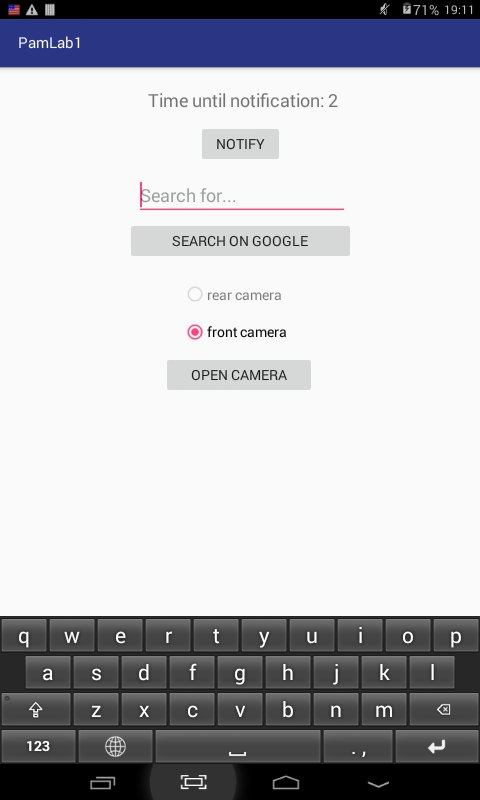
\includegraphics[width=4cm]{s2.jpg}
        \label{fig:s1}
        \caption{Notification button was pressed}
        \end{figure}

        The same way, in the figure 2 we notice the notification which has appeared in the notification bar.

        \begin{figure}[h]
        \centering
        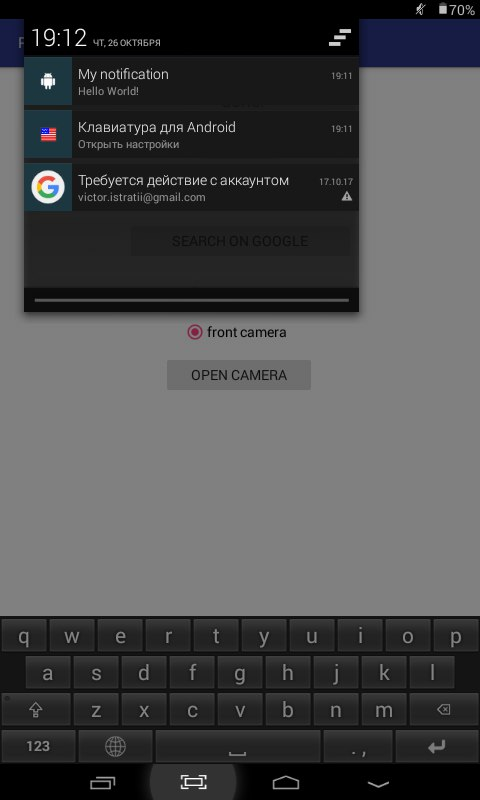
\includegraphics[width=4cm]{s3.jpg}
        \label{fig:s2}
        \caption{Notification button was pressed}
        \end{figure}

    \newpage

    \section*{Task 2}
        The task with google search may seem difficult at first sight, but is solved very fastly. What I had to do was only to create a corresponding intent, specifying the correct attribute on creation, Intent.ACTION\_VIEW and giving it the respective uri, created from parsing "https://www.google.com/search?q=" + user input. 

        In figure 3 we see the google search results in the browser, after one has pressed the search button in the activity.

        \begin{figure}[h]
        \centering
        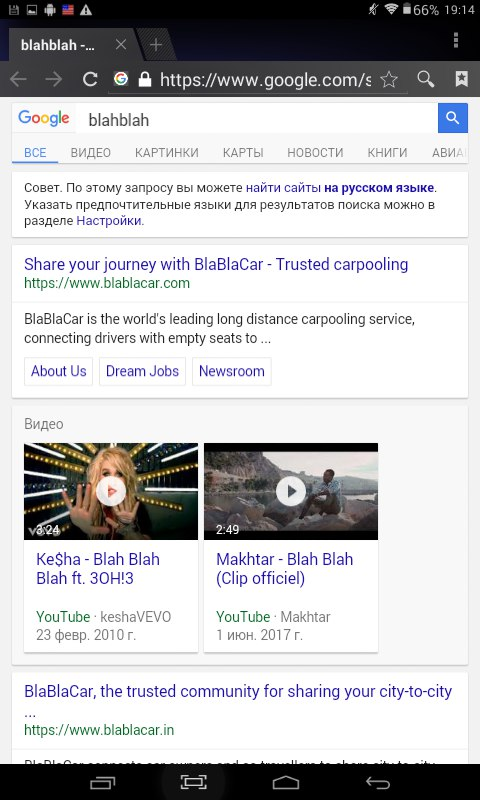
\includegraphics[width=6cm]{s4.jpg}
        \label{fig:s3}
        \caption{Result of searching from app}
        \end{figure}

    \section*{Task 3}
        When working with the camera, a difficulty was to determine which cameras are present on the device. For example, my tablet has only the frontal camera, thus it was necessary to check which cameras does the device have. I've defined 2 functions. One of them uses the PackageManager to check is the frontal is present and the other checks the back camera by using the old Camera api.
        \\\\
        Next, I have defined a radiogroup with 2 radios for each camera. Depending on the present cameras, one or another radiobuttons can be disabled. After choosing one and pressing the button, an intent is fired and the respective camera is opened.

    \section*{Task 4}
        To solve this task I needed some way to handle the image capturing event. The handling was combined with the functionality of launching the camera from button. In such a way, in the button listener I defined an intent, which would be launched as activity result - meaning that after one takes and saves a picture, an intent will be fired. The behavior is defined in the function onActivityResult(), where I create the intent for a new activity, add to its data the taken image and launch the activity.

        The result can be seen in fig 3 and 4:

        \begin{figure}[h]
        \centering
        \begin{minipage}{.5\textwidth}
          \centering
          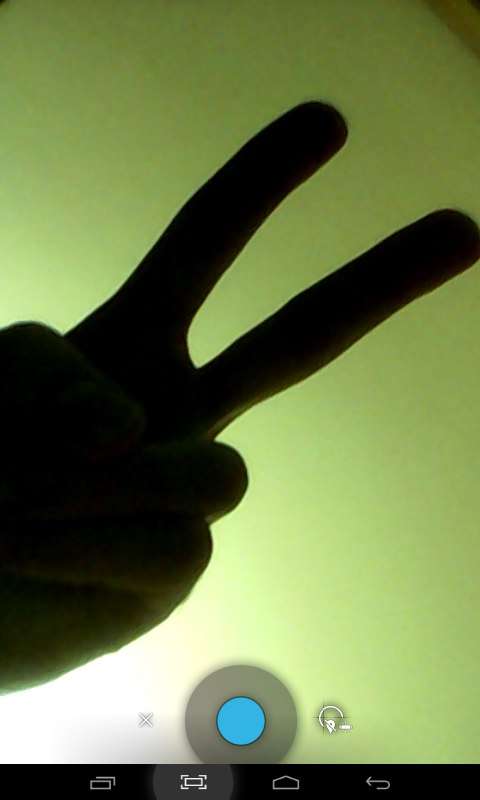
\includegraphics[width=.4\linewidth]{s5.jpg}
          \caption{Taking the picture}
        \end{minipage}%
        \begin{minipage}{.5\textwidth}
          \centering
          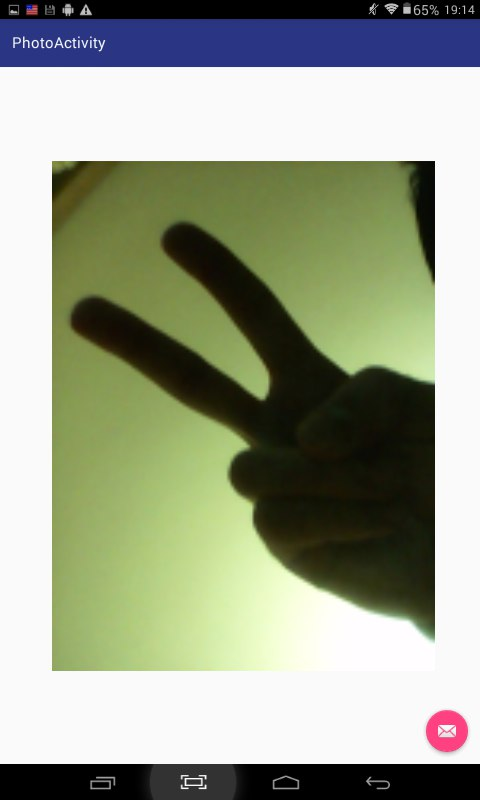
\includegraphics[width=.4\linewidth]{s6.jpg}
          \caption{The picture displayed}
        \end{minipage}
        \end{figure}


    \section*{Conclusion}
        In this laboratory work we have got a strong insight about Android intents. So, basically, an intent is an abstract description of an operation to be performed. It provides a facility for performing late runtime binding between the code in different applications. Its most significant use is in the launching of activities, where it can be thought of as the glue between activities. It is basically a passive data structure holding an abstract description of an action to be performed.
        \\\\
        We have learned that the intents are quite powerful in terms of working with activities, however they can become bulky and slow down the application, when it comes to transmitting large amounts of data.






\end{document}